\documentclass[a4paper,12pt]{article}
\usepackage{amsmath,amssymb,amsfonts,amsthm}
\usepackage{tikz}
\usepackage [utf8x] {inputenc}
\usepackage [T2A] {fontenc} 
\usepackage[russian]{babel}
\usepackage{cmap, upgreek}
\usepackage{textcomp} 

% Так ссылки в PDF будут активны
\usepackage[unicode]{hyperref}

% вы сможете вставлять картинки командой \includegraphics[width=0.7\textwidth]{ИМЯ ФАЙЛА}
% получается подключать, как минимум, файлы .pdf, .jpg, .png.
\usepackage{graphicx}
% Если вы хотите явно указать поля:
\usepackage[margin=1in]{geometry}
% Или если вы хотите задать поля менее явно (чем больше DIV, тем больше места под текст):
% \usepackage[DIV=10]{typearea}

\usepackage{fancyhdr}

\newcommand{\bbR}{\mathbb R}%теперь вместо длинной команды \mathbb R (множество вещественных чисел) можно писать короткую запись \bbR. Вместо \bbR вы можете вписать любую строчку букв, которая начинается с '\'.
\newcommand{\eps}{\varepsilon}
\newcommand{\bbN}{\mathbb N}
\newcommand{\dif}{\mathrm{d}}

\newtheorem{Def}{Определение}


\pagestyle{fancy}
\makeatletter % сделать "@" "буквой", а не "спецсимволом" - можно использовать "служебные" команды, содержащие @ в названии
\fancyhead[L]{\footnotesize Электричество и магнетизм}%Это будет написано вверху страницы слева
\fancyhead[R]{\footnotesize ФМХФ МФТИ}
\fancyfoot[L]{\footnotesize \@author}%имя автора будет написано внизу страницы слева
\fancyfoot[R]{\thepage}%номер страницы —- внизу справа
\fancyfoot[C]{}%по центру внизу страницы пусто

\renewcommand{\maketitle}{%
	\noindent{\bfseries\scshape\large\@title\ \mdseries\upshape}\par
	\noindent {\large\itshape\@author}
	\vskip 2ex}
\makeatother
\def\dd#1#2{\frac{\partial#1}{\partial#2}}


\title{3.5.1 \\ Изучение плазмы газового разряда в неоне}
\author{Егор Берсенев} 
\date{15 апреля 2016 г.}

\begin{document}
	\maketitle
	\section{Цель работы}
		 Изучение ВАХ тлеющего разряда, изучение свойств плазмы методом зондовых характеристик.
	\section{Оборудование}
		Стеклянная газоразрядная трубка, наполненная изотопом неона, высоковольтный источник питания, источник постоянного тока, делитель напряжения, резистор, потенциометр, амперметры, вольтметры, переключатели.
	\section{Теоретическая часть}
		Схема установки представлена на рисунке \ref{pic:1}. Стеклянная газоразрядная трубка имеет холодный полый катод, три анода и геттерный узел --- стеклянный баллон, на внутреннюю поверхность которого напылена газопоглощающая пленка. Трубка наполнена $^{22}\mathbf{Ne}$ при давлении 2 мм рт.ст. Катод и один из анодов с помщью переключателя $\text{П}_1$ подключаются через балластный резистор $R_{\text{б}}\simeq 450\, \text{кОм}$ к регулируемому высоковольтному источнику питания с выходным напряжением до 3 кВ.
		\begin{figure}[h]
			\centering
			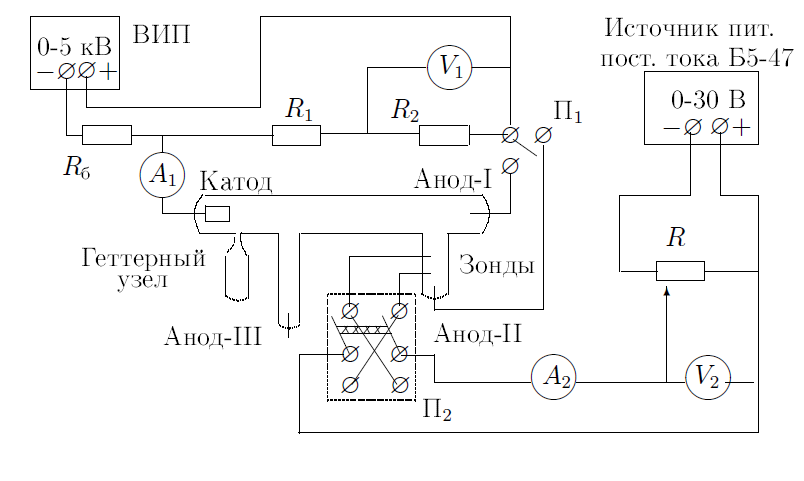
\includegraphics[width = 0.7\linewidth]{pic1}
			\caption{Схема установки для исследования газового разряда}
			\label{pic:1}
		\end{figure}
		
		При подключении к ВИП анода-I между ним и катодом возникает газовый разряд. Ток разряда измеряется миллиамперметром $\mathrm{A}_1$, а падение напряжения на разрядной трубке --- цифровым вольтметром $\mathrm{V}_1$, подключенным к трубке через высокоомный делитель напряжения с коэффициентом $\cfrac{R_1+R_2}{R_2} = 10\,\text{Ом}$ 
			
		При подключении к ВИП анода-II разряд возникает в пространстве, где находится двойной зонд, используемый для диагностики плазмы положительного столба. Зонды изготовлены из молибденовой проволоки диаметром $d = 0.2\,\text{мм}$ и имеют длину $l = 5.2\,\text{мм}$. Они подключены к источнику питания через потенциометр $\mathrm{R}$. Переключатель $\text{П}_2$ позволяет изменять полярность напряжения на зондах. Величина напряжения на зондах изменяется  с помощью дискретного переключателя <<$\mathrm{V}$>> выходного напряжения источника питания и потенциометра, а измеряется вольтметром $\mathrm{V}_2$. Для измерения зондового тока используется микроамперметр $\mathrm{A}_2$.
		
		\section{Ход работы}
		\subsection{Вольт-амперная характеристика разряда}
		
		\begin{table}[h]
			\centering
			\caption{Вольт-амперная характеристика разряда}
			\label{my-label}
			\begin{tabular}{|l|l|l|l|l|l|l|l|l|}
				\hline
				U, В & 25.46 & 25.78 & 25.92 & 26.22 & 26.31 & 26.5  & 26.66 & 26.85 \\ \hline
				I, мА & 5     & 4.68  & 4.44  & 4.28  & 4.2   & 4.08  & 4     & 3.88  \\ \hline
				U, В & 27.08 & 27.28 & 27.53 & 27.82 & 27.97 & 28.3  & 28.4  & 28.53 \\ \hline
				I, мА & 3.8   & 3.68  & 3.56  & 3.48  & 3.4   & 2.8   & 3.2   & 2.72  \\ \hline
				U, В & 28.75 & 29.08 & 29.7  & 30.58 & 31.33 & 31.63 & 32.45 & 32.72 \\ \hline
				I, мА & 2.92  & 2.56  & 2.4   & 2.2   & 2.08  & 2     & 1.8   & 1.6   \\ \hline
				U, В & 33.05 & 33.42 & 33.9  & 34.24 & 34.34 & 34.78 & 35.14 & 35.84 \\ \hline
				I, мА & 1.4   & 1.2   & 1     & 0.92  & 0.8   & 0.6   & 0.4   & 0.2   \\ \hline
			\end{tabular}
		\end{table}
		
		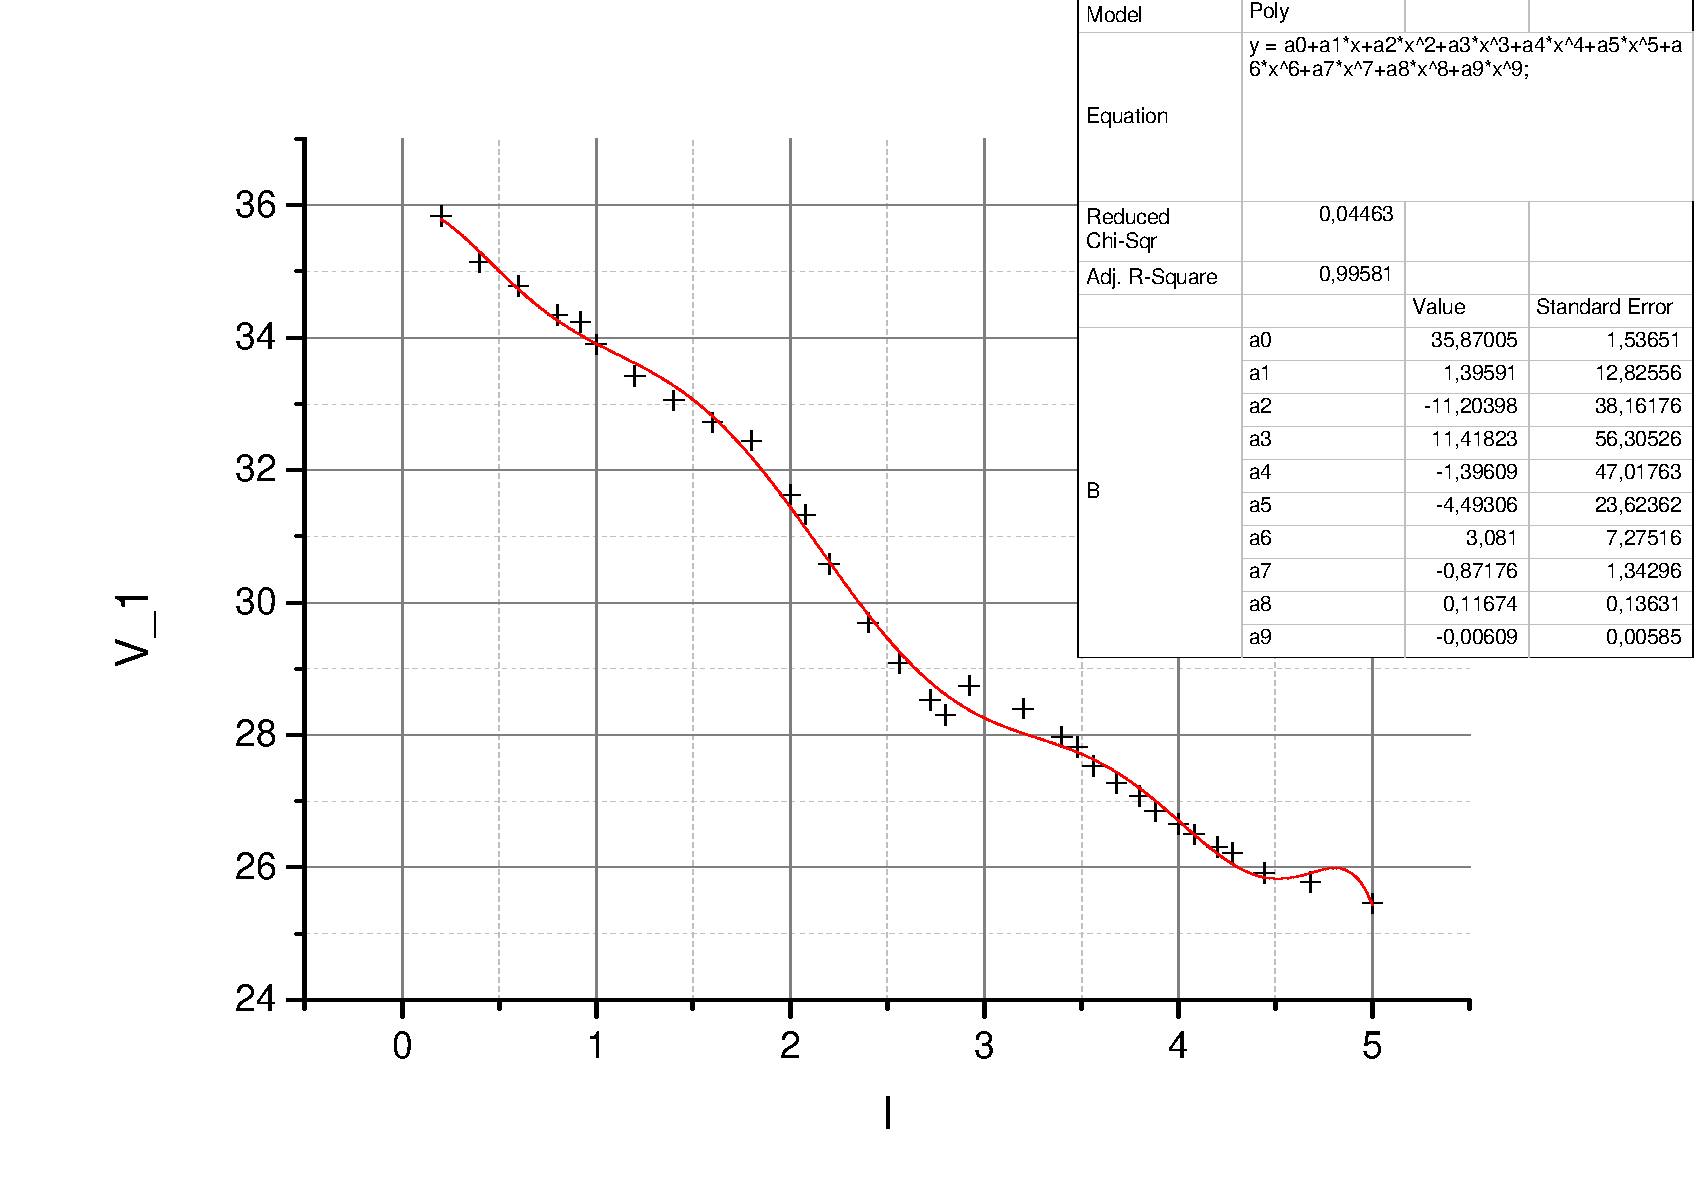
\includegraphics[width = \linewidth]{graph1}
		
		$R^\dif_{max} = -5.325\cdot10^{3}$ Ом.
		
		
		\subsection{Зондовые характеристики}
		
		\begin{table}[h]
			\centering
			\caption{Зондовые характеристики разряда}
			\label{my-label}
			\begin{tabular}{|l|l|l|l|l|l|}
				\hline
				\multicolumn{2}{|l|}{I = 5 mA} & \multicolumn{2}{l|}{I = 3.6 mA} & \multicolumn{2}{l|}{I = 1.4 mA} \\ \hline
				I          & U         & I         & U         & I         & U         \\ \hline
				-95,6      & -25,05    & -65,67    & -25,05    & -25,37    & -25,05    \\ \hline
				-93,24     & -22,03    & -63,74    & -22       & -24,5     & -22       \\ \hline
				-90,63     & -19,01    & -61,94    & -19       & -23,62    & -19,02    \\ \hline
				-86,92     & -16,02    & -59,82    & -16,01    & -22,7     & -16       \\ \hline
				-81,12     & -13       & -56,61    & -13,02    & -21,54    & -13       \\ \hline
				-72        & -10,01    & -50,77    & -10       & -19,47    & -10       \\ \hline
				-63,36     & -8,01     & -44,8     & -8        & -17,27    & -8,01     \\ \hline
				-52,4      & -6,01     & -36,7     & -6        & -14,19    & -6        \\ \hline
				-32,12     & -3,01     & -29,59    & -4        & -10,22    & -4        \\ \hline
				-30,31     & -4,01     & -20,81    & -3        & -7,82     & -2,98     \\ \hline
				-28,19     & -2,49     & -17,88    & -2,25     & -6,61     & -2,5      \\ \hline
				-24,59     & -2,01     & -14,8     & -2,01     & -5,34     & -2        \\ \hline
				-20,62     & -1,5      & -11,59    & -1,5      & -4,07     & -1,51     \\ \hline
				-16,78     & -1        & -8,47     & -1,02     & -2,65     & -0,99     \\ \hline
				-12,91     & -0,5      & -5,12     & -0,49     & -1,38     & -0,51     \\ \hline
				14,76      & 0,5       & 6,54      & 0,49      & 1,7       & 0,47      \\ \hline
				18,55      & 1         & 9,82      & 1,02      & 3,09      & 1         \\ \hline
				22,25      & 1,48      & 12,68     & 1,48      & 4,41      & 1,5       \\ \hline
				26,22      & 2         & 16,06     & 2,02      & 5,69      & 2         \\ \hline
				29,9       & 2,5       & 18,85     & 2,5       & 6,94      & 2,5       \\ \hline
				33,84      & 3,02      & 21,6      & 2,97      & 8,15      & 3,01      \\ \hline
				40,65      & 4         & 27,16     & 4         & 10,29     & 3,99      \\ \hline
				52,95      & 6,02      & 36,55     & 6         & 14,14     & 6,06      \\ \hline
				62,57      & 8         & 43,82     & 8         & 16,86     & 8         \\ \hline
				70,05      & 10,02     & 49,08     & 10,03     & 18,87     & 9,97      \\ \hline
				77,46      & 13        & 53,9      & 13,04     & 20,63     & 12,98     \\ \hline
				82         & 16,08     & 56,79     & 16        & 21,68     & 15,99     \\ \hline
				84,77      & 19        & 58,62     & 19,03     & 22,55     & 19,04     \\ \hline
				87         & 22,01     & 60,32     & 22,02     & 23,4      & 22,03     \\ \hline
				89,08      & 25,05     & 61,99     & 25,05     & 24,24     & 25,05     \\ \hline
			\end{tabular}
		\end{table}
		
		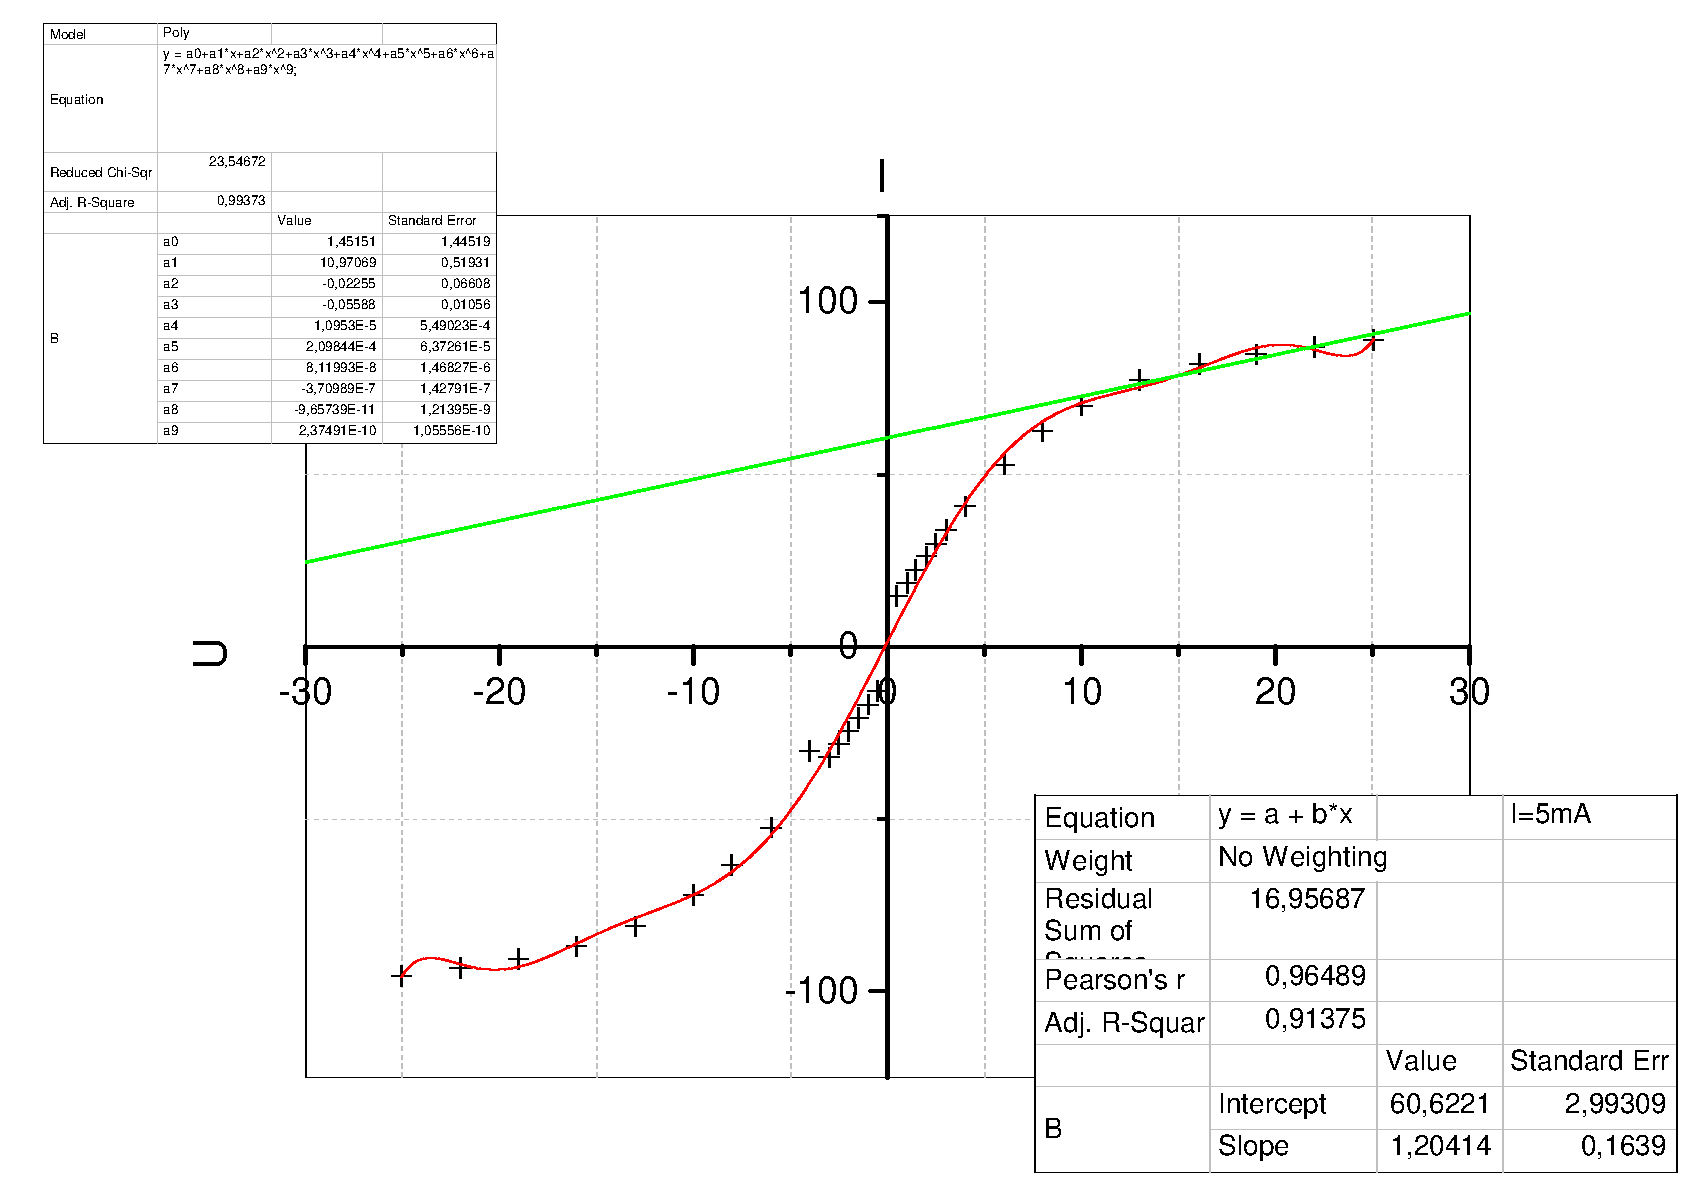
\includegraphics[width = \linewidth]{5mA}
		
		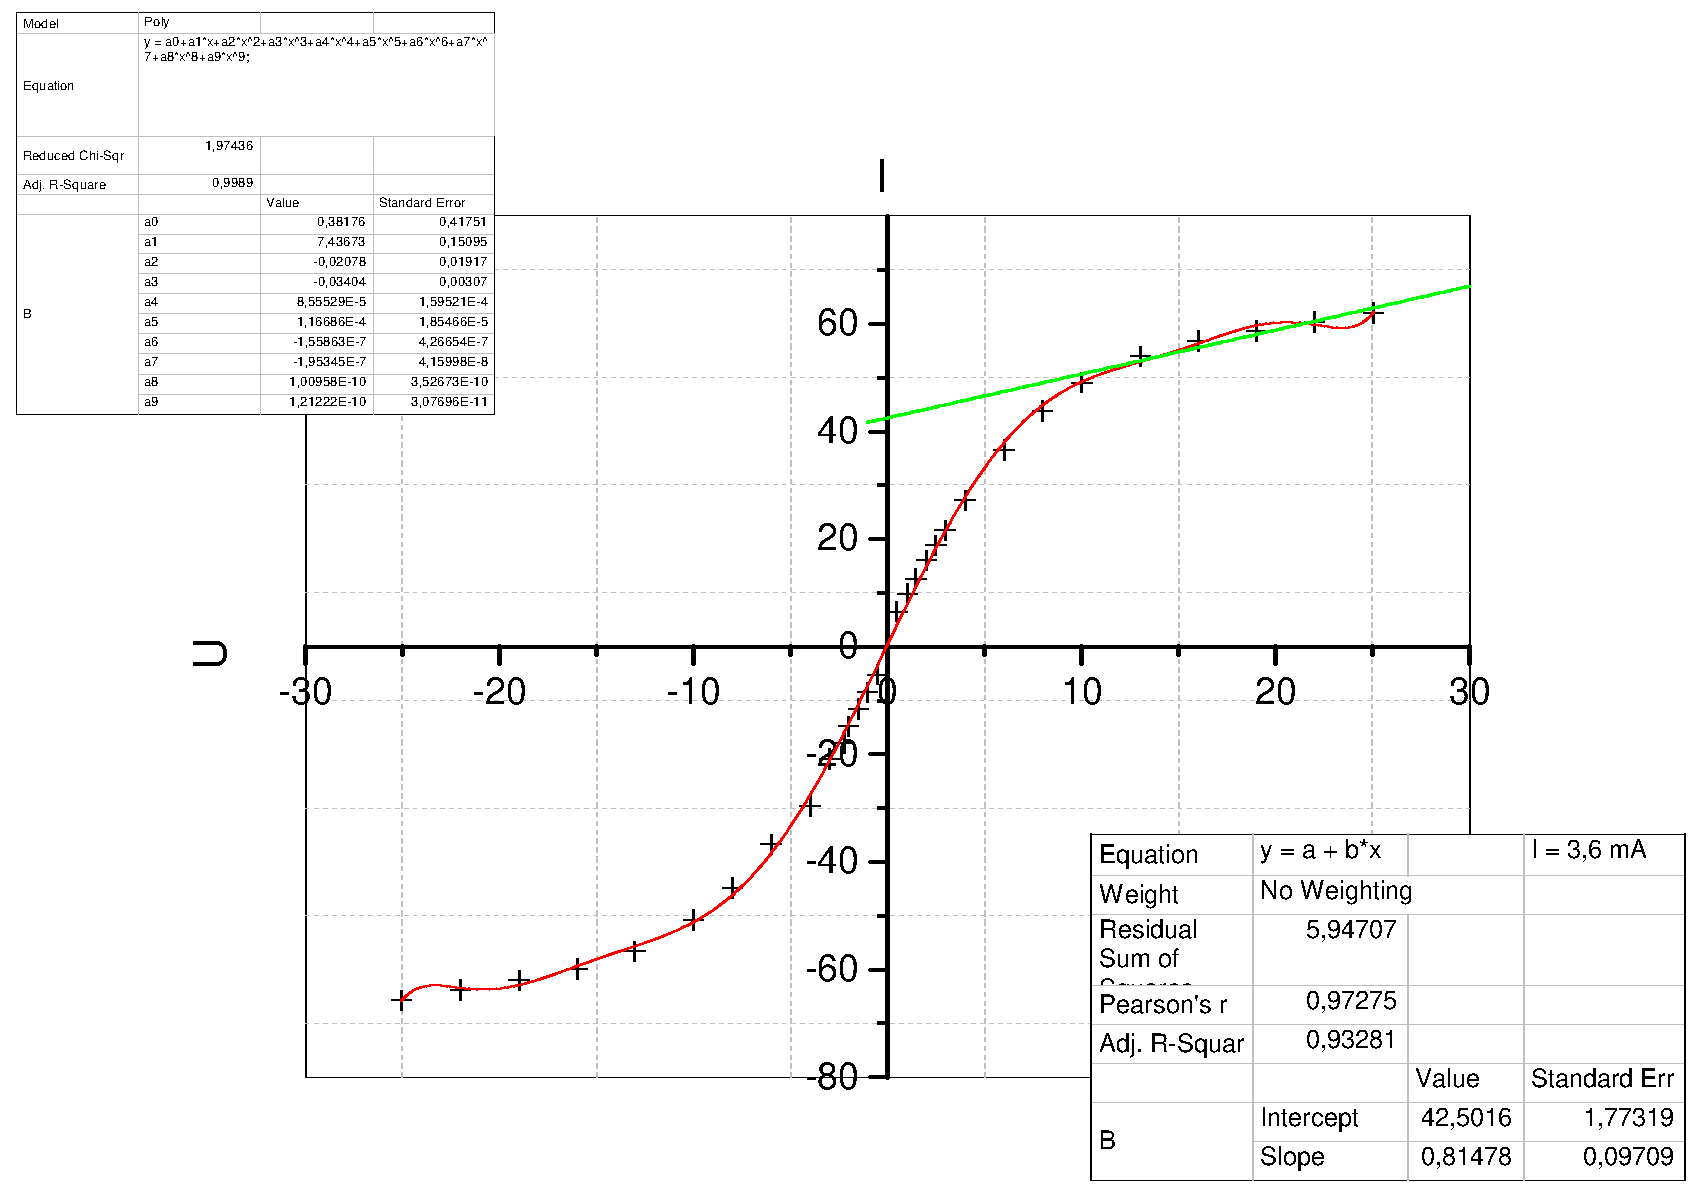
\includegraphics[width = \linewidth]{36mA}
		
		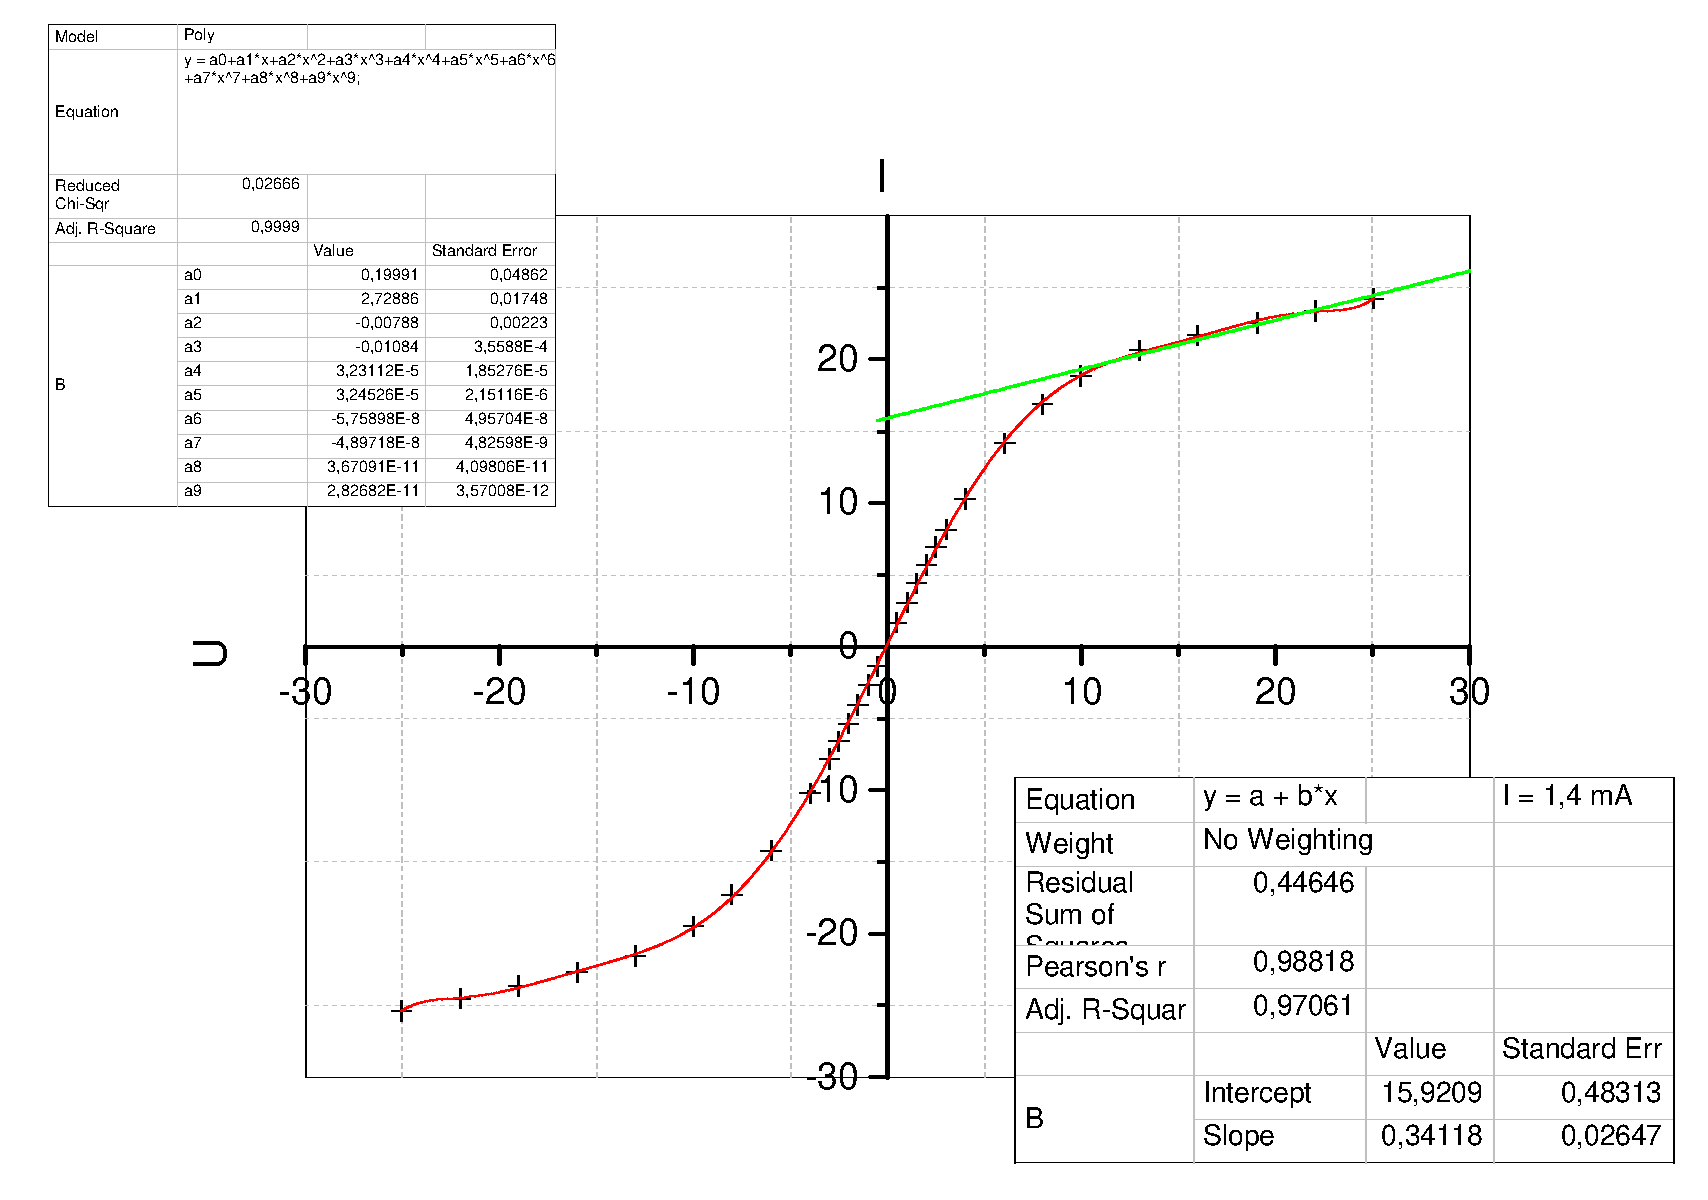
\includegraphics[width = \linewidth]{14mA}
		
		
		\begin{table}[h]
			\centering
			\caption{Результаты экспериментов}
			\label{my-label}
			\begin{tabular}{|l|l|l|l|}
				\hline
				$I_r$, мА     & 1.4   & 3.6   & 5     \\ \hline
				$\frac{\dif I}{\dif U}$  & 2.76  & 9.08  & 17.67 \\ \hline
				$I_{in}$  & 15.92 & 42.5  & 60.62 \\ \hline
				$kT$, эВ    & 2.89  & 2.81  & 2.72  \\ \hline
				$n_e\cdot 10^{13}$, 1/м$^3$    & 1.9   & 5.64  & 9.4   \\ \hline
				$\omega\cdot 10^{6}$, 1/c & 245.9 & 423.3 & 547   \\ \hline
				$r_d\cdot 10^{-3}$     & 26    & 15    & 11.7  \\ \hline
			\end{tabular}
		\end{table}
		
		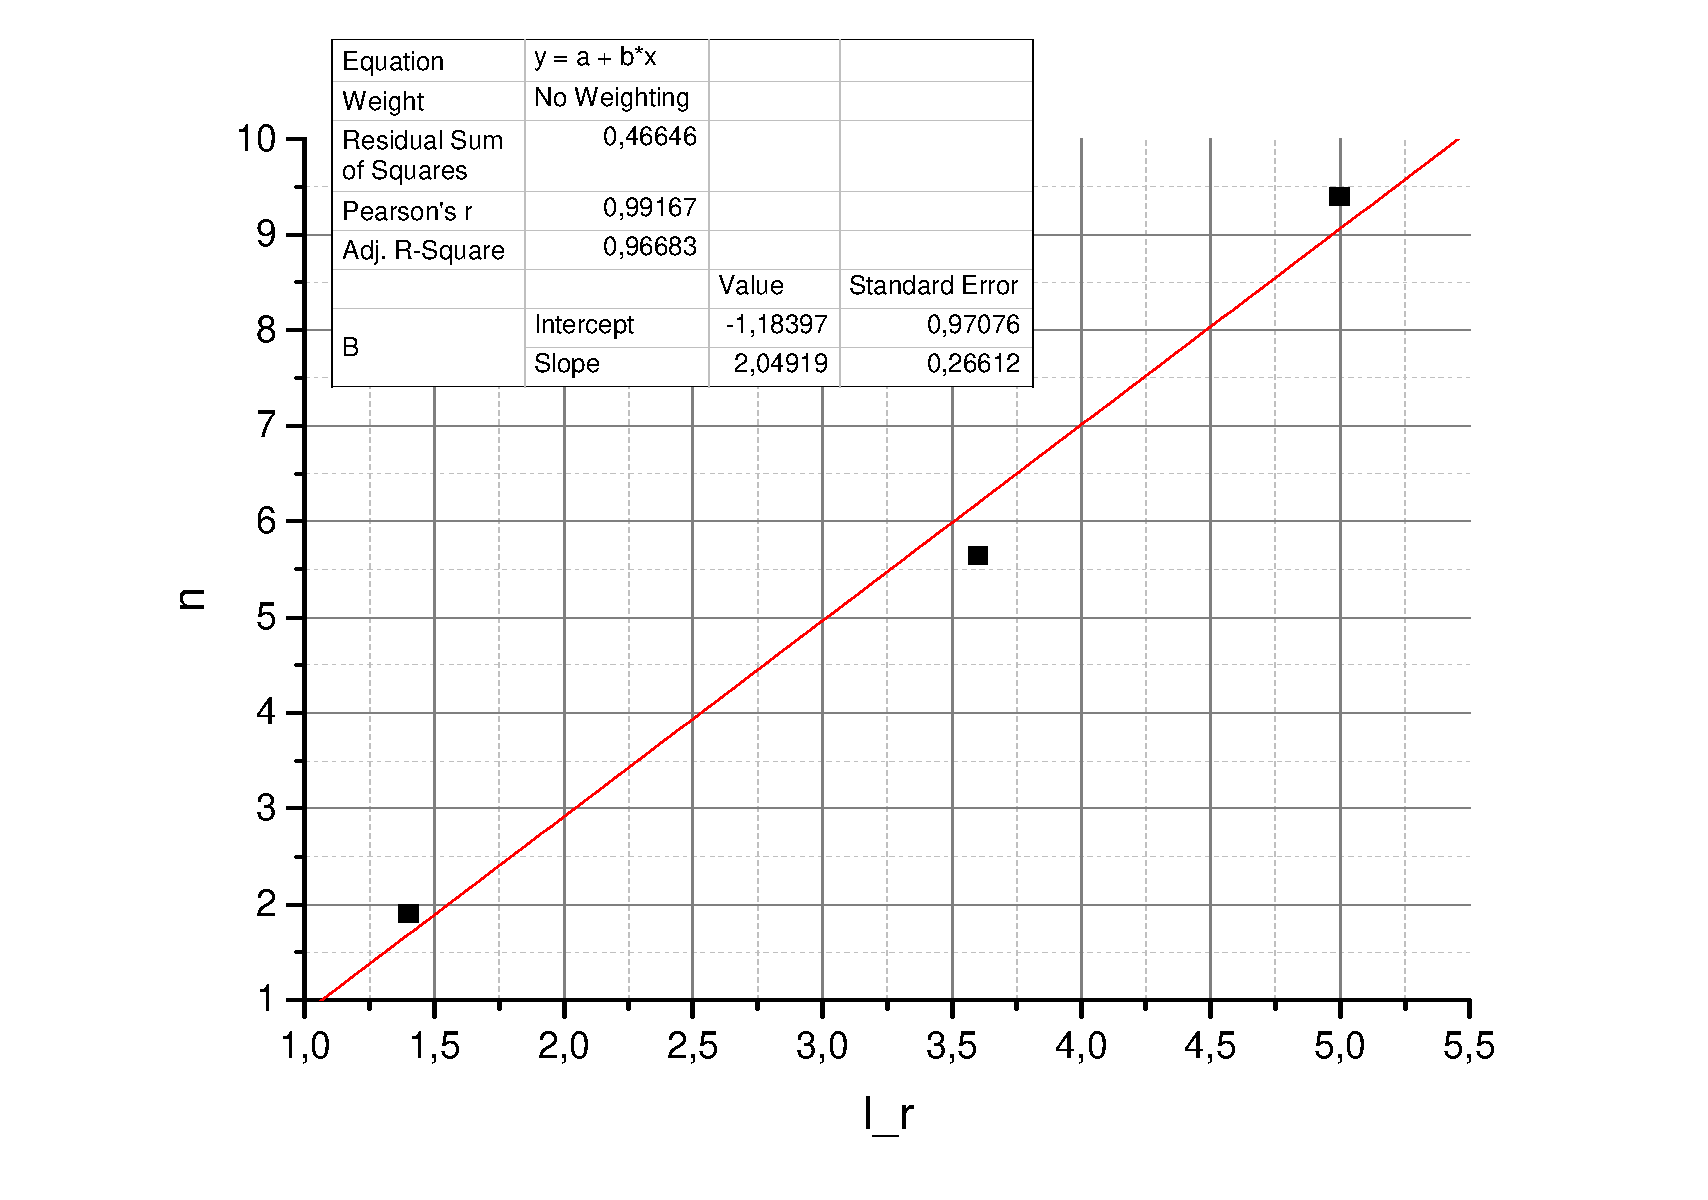
\includegraphics[width=0.7\linewidth]{ni} 

		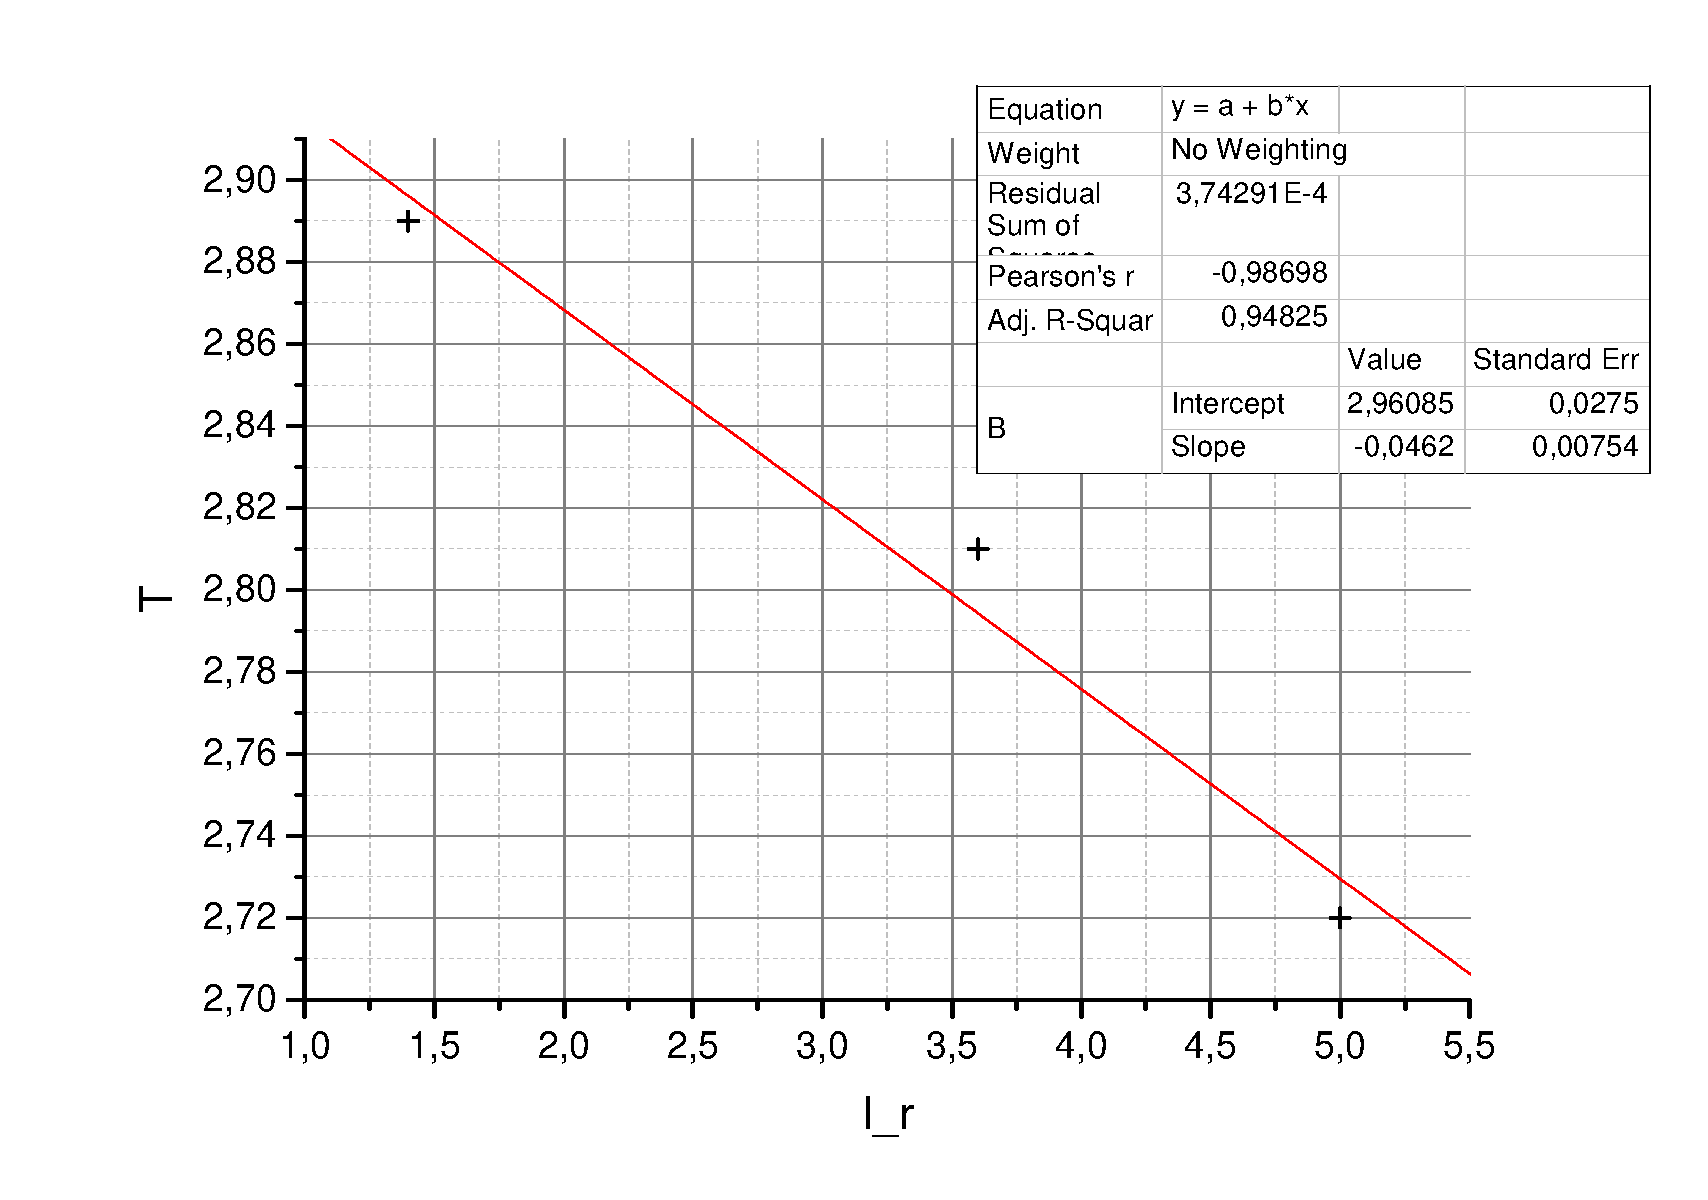
\includegraphics[width=0.7\linewidth]{ti} 

		
		\section{Вывод}
			Исследуя плазму газового разряда в неоне с помощью зонда, можно рассчитать температуру и концентрацию как ионов, так и электронов.
		
\end{document}


